%% Section 6: Firm-Level Results

\section{Firm-Level Results}
\label{sec:results_micro}

\subsection{Enterprise Outcomes: NLPS Panel}
\label{sub:nlps_results}

Figure~\ref{fig:eventstudy_firm} plots the round-specific
$\textit{Fintech}_s \times \text{round}$ coefficients for enterprise survival
on a calendar timeline. The enterprise module was fielded only in Rounds~5, 7,
and~11, so firm-level pre-trends cannot be tested directly. The \NTL{}
pre-trend validation in Section~\ref{sub:pretrendvalid} addresses this gap as
 the treatment variable $\textit{Fintech}_s$ is identical across the
\NTL{} and firm specifications, the 45-month pre-shock test of whether
$\textit{Fintech}_s$ predicts differential \NTL{} trajectories constitutes a
direct test of the parallel-trends assumption for the firm panel as well.
That the pre-period coefficients are statistically
indistinguishable from zero, together with enterprise fixed effects that absorb
all time-invariant enterprise heterogeneity, supports the validity of the
estimates below.

The figure shows two patterns that are central to the paper's argument. First,
the enterprise survival differential is statistically positive at the peak
crunch (Round~7, February 2023), consistent with an insulation effect
concentrated at the height of the cash shortage. Second, the differential
\emph{widens} to 7.7 percentage points by the medium run (Round~11,
April 2024), with confidence intervals lying entirely above zero. This
widening rules out a transitory disruption notion, under which the crunch
temporarily disadvantaged low-fintech enterprises but the gap closed after
normalisation, and instead suggests that the cash supply shock triggered
persistent enterprise exit in low-fintech states.

\begin{figure}[H]
\centering
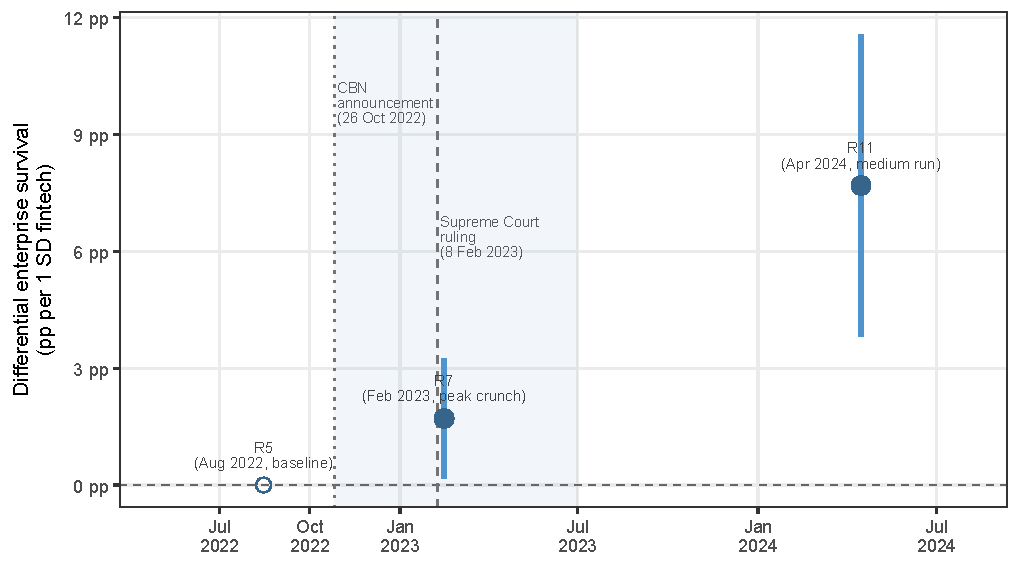
\includegraphics[width=0.94\textwidth]{figures/fig_eventstudy_firm.pdf}
\refstepcounter{figure}\label{fig:eventstudy_firm}
\floatfoot{%
  \textit{Notes:} Round-specific DiD coefficients from
  equation~\eqref{eq:firm}, plotting the differential enterprise survival
  probability (in percentage points) per one standard deviation of
  pre-shock fintech adoption ($\textit{Fintech}_s$).
  Round~5 (August 2022, pre-shock baseline) is the reference category
  (open circle, coefficient $= 0$ by construction).
  Solid circles are estimated coefficients; vertical bars are 95\%
  confidence intervals based on standard errors clustered at the
  state level. Shading marks the naira crunch window (CBN announcement
  to approximate cash normalisation). Dotted and dashed vertical lines
  mark the CBN announcement (26~October 2022) and Supreme Court ruling
  (8~February 2023) respectively. The \NLPS{} enterprise module was
  fielded only in Rounds~5, 7, and~11; there are no pre-shock
  enterprise observations.
}
\end{figure}

Table~\ref{tab:firm_did} presents estimates of equation~\eqref{eq:firm} for
three outcomes: an indicator for enterprise activity during the survey week
(columns 1--2), log weekly sales (columns 3--4), and the number of enterprise
workers (column 5). Odd columns omit sector and household controls; even
columns include them.

\begin{table}[H]
\caption{Firm-Level Effects of the Naira Crunch}
\label{tab:firm_did}

\begingroup
\centering
\begin{tabular}{lccccc}
   \tabularnewline \midrule \midrule
    & \multicolumn{2}{c}{Active} & \multicolumn{2}{c}{Log sales} & Workers \\ 
   Dependent Variables: & \multicolumn{2}{c}{active} & \multicolumn{2}{c}{ln\_sales} & n\_workers\\
   Model:                             & (1)            & (2)            & (3)            & (4)            & (5)\\  
   \midrule
   \emph{Variables}\\
   Fintech $\times$ R7 (peak crunch)  & 0.0171$^{**}$  & 0.0171$^{**}$  & 0.0184         & 0.0184         & 0.2940$^{***}$\\   
                                      & (0.0076)       & (0.0076)       & (0.0847)       & (0.0847)       & (0.0550)\\   
   Fintech $\times$ R11 (medium run)  & 0.0769$^{***}$ & 0.0769$^{***}$ & 0.3149$^{***}$ & 0.3149$^{***}$ &   \\   
                                      & (0.0192)       & (0.0192)       & (0.0925)       & (0.0925)       &   \\   
   Enterprise FE                      & \checkmark     & \checkmark     & \checkmark     & \checkmark     & \checkmark\\   
   Round FE                           & \checkmark     & \checkmark     & \checkmark     & \checkmark     & \checkmark\\   
   Rural control                      & No             & Yes            & No             & Yes            & No\\  
   \midrule
   \emph{Fixed-effects}\\
   hh\_f                              & Yes            & Yes            & Yes            & Yes            & Yes\\  
   round                              & Yes            & Yes            & Yes            & Yes            & Yes\\  
   \midrule
   \emph{Fit statistics}\\
   Observations                       & 5,269          & 5,269          & 3,482          & 3,482          & 3,084\\  
   R$^2$                              & 0.68987        & 0.68987        & 0.42580        & 0.42580        & 0.51830\\  
   Within R$^2$                       & 0.01309        & 0.01309        & 0.00530        & 0.00530        & 0.03387\\  
   \midrule \midrule
   \multicolumn{6}{l}{\emph{Clustered (state\_f) standard-errors in parentheses}}\\
   \multicolumn{6}{l}{\emph{Signif. Codes: ***: 0.01, **: 0.05, *: 0.1}}\\
\end{tabular}
 
\par \raggedright 
Sample: non-farm household enterprises active in NLPS Round 5 (August 2022 pre-shock baseline). Round 5 is the omitted baseline. Fintech is the standardised state-level digital payment index from NLPS Round 6 (October 2022). Workers only available for R5 and R7. Standard errors clustered at the state level. Inference robustness: see Appendix Table~\ref{atab:inference_robustness}.
\par\endgroup



\end{table}

Table~\ref{tab:firm_did} reports the main firm-level results. Enterprises in states one standard
deviation above the pre-shock fintech mean were 1.7 percentage points more
likely to remain in operation at the February 2023 peak crunch
($\hat\delta_{R7} = 0.017$, $p = 0.030$). Appendix
Table~\ref{atab:inference_robustness} reports inference under pairs bootstrap
and randomisation inference; under randomisation inference the R7 survival
effect is significant at the 10\% level ($p_{\text{RI}} = 0.085$), while the
R11 survival and R7 employment results remain significant at the 1\% level
under all inference methods. The R7 result should therefore be read as
suggestive support of the peak-crunch insulation channel, with R11
survival and employment providing the bedrock evidence. By April 2024 (Round~11, 14~months post-peak), 
the survival advantage has \emph{widened} to 7.7 percentage points ($p < 0.001$), indicating that the
initial resilience compounded into a durable medium-run advantage rather than
dissipating.

Employment results shows that enterprises in high-fintech states
had 0.29 more workers at peak crunch per standard deviation of fintech
($p < 0.001$). Log weekly sales at peak crunch (R7) are positive (0.018) but
statistically indistinguishable from zero ($p = 0.83$). A plausible
explanation is positive survivor selection in low-fintech states such that enterprises
that \emph{remained open} in low-fintech states at R7 were positively selected
on productivity, only the most efficient firms survived, compressing the
observable sales differential among survivors. Appendix
Table~\ref{atab:sales_decomp} provides formal evidence for this mechanism, where
pre-shock (R5) log sales are 0.162 log points higher among R7-survivors than
exiters in the low-fintech tercile, but 0.475 points \emph{lower} among
survivors versus exiters in the high-fintech tercile, confirming that
low-fintech survivors constitute a positively selected sub-sample.

On the other hand, the medium-run log-sales coefficient at R11 is large and
significant, $\hat\delta_{R11} = 0.315$ ($p < 0.001$), indicating
approximately 37\% higher weekly sales in high-fintech states fourteen months
after the peak. The R11 log-sales regression conditions on survival to
Round~11; that is, the comparison is restricted to enterprises that remained
active in both high- and low-fintech states. By April~2024, additional exit in
low-fintech states between R7 and R11 has depleted even the positively-selected
survivors identified at R7, leaving a residual sample that is thinner and
drawn from the lower tail of the low-fintech productivity distribution. The
widening sales gap at R11 therefore suggests the \emph{compounding} of two
forces: a genuine long-run divergence in productivity between enterprises that
maintained sales relationships and supplier networks through the crunch, and a
composition effect as continued exit in low-fintech states erodes the
survivor-selection buffer that suppressed the gap at R7. Both forces are indicative of a
persistent real cost of cash supply shocks in states with weak digital
infrastructure.

The medium-run survival gap at R11, 7.7 percentage points, is particularly noteworthy. 
The 16-percentage-point decline in enterprise activity from R5 to
R11 was not equally distributed as it was concentrated in low-fintech states
where the crunch proved a permanent exit shock for many small enterprises.

\subsection{Heterogeneity}
\label{sub:heterogeneity}

Table~\ref{tab:heterogeneity} presents two heterogeneity dimensions. Rural
versus urban location, and small versus large enterprises (split at the median
baseline worker count). The fintech insulation effect is concentrated in rural
enterprises (R7 coefficient of 0.026, $p = 0.015$) and small enterprises
(0.038, $p = 0.019$), while the urban and large-enterprise coefficients are
smaller and not statistically significant. This gradient is consistent with
the underlying mechanism that rural and small enterprises are more exclusively
dependent on physical cash for both receipts and payments, with fewer access
points to POS machines or formal banking buffers. Large urban enterprises
are better diversified across payment channels, reducing the marginal benefit
of state-level fintech infrastructure.

\begin{table}[H]
\caption{Heterogeneity by Location and Firm Size}
\label{tab:heterogeneity}

\begingroup
\centering
\begin{tabular}{lcccc}
   \tabularnewline \midrule \midrule
                                      & Rural          & Urban          & Small          & Large \\   
   Dependent Variable: & \multicolumn{4}{c}{active}\\
   Model:                             & (1)            & (2)            & (3)            & (4)\\  
   \midrule
   \emph{Variables}\\
   Fintech $\times$ R7 (peak crunch)  & 0.0263$^{**}$  & 0.0004         & 0.0379$^{**}$  & -0.0065\\   
                                      & (0.0103)       & (0.0134)       & (0.0154)       & (0.0099)\\   
   Fintech $\times$ R11 (medium run)  & 0.0771$^{***}$ & 0.0700$^{***}$ & 0.0750$^{***}$ & 0.0698$^{***}$\\   
                                      & (0.0212)       & (0.0188)       & (0.0209)       & (0.0245)\\   
   \midrule
   \emph{Fixed-effects}\\
   hh\_f                              & Yes            & Yes            & Yes            & Yes\\  
   round                              & Yes            & Yes            & Yes            & Yes\\  
   \midrule
   \emph{Fit statistics}\\
   Observations                       & 3,765          & 1,504          & 2,497          & 2,772\\  
   R$^2$                              & 0.67312        & 0.73562        & 0.67448        & 0.70521\\  
   Within R$^2$                       & 0.01137        & 0.01629        & 0.01201        & 0.01309\\  
   \midrule \midrule
   \multicolumn{5}{l}{\emph{Clustered (state\_f) standard-errors in parentheses}}\\
   \multicolumn{5}{l}{\emph{Signif. Codes: ***: 0.01, **: 0.05, *: 0.1}}\\
\end{tabular}
 
\par \raggedright 
Dependent variable: enterprise active (binary). Split-sample estimates. Small = below-median workers at R5 baseline. Standard errors clustered at state level.
\par\endgroup



\end{table}
